\nopagebreak
\section{theory}
\subsection{Plane parallel layer}
The investigated semiconductor samples can in first approximation be described as a plane parallel 
layer with a thickness $d$ and refractive index $N_2$ which acts like a fabry-perot interferometer.
\begin{figure}[h]
    \centering
    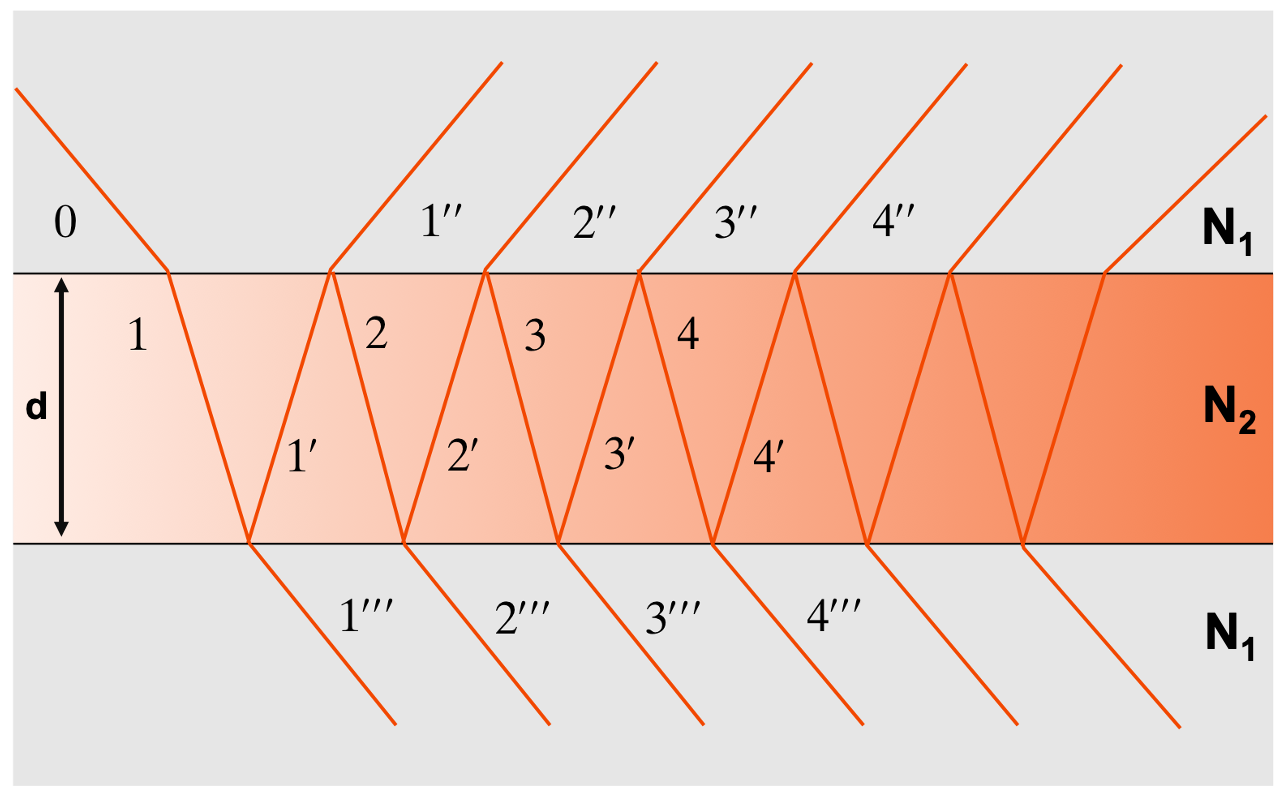
\includegraphics[width=0.5\textwidth]{Fabry-Perot.png}
    \caption{Simplified illustration of the measured samples as a plane parallel plate
    with thickness $d$ and refractive index $N_2$. The surrounding air is described with a 
    refractive indes $N_1\approx1$ \cite{Gerthsen}}
    \label{fig:layer}
\end{figure}
